\documentclass[11.5pt]{article}
\usepackage{chatsagnik}
% \usepackage[shortlabels]{enumitem}
\setitemize{noitemsep,topsep=3pt,parsep=2pt,partopsep=2pt} 
\setenumerate{itemsep=1pt,topsep=2pt,parsep=2pt,partopsep=2pt}
\setdescription{itemsep=1pt}

\author[1]{Sagnik Chatterjee}
\affil[1]{Indraprashta Institute of Information Technology (IIIT-D), Delhi, India}
\affil[ ]{\textit {\{sagnikc\}@iiitd.ac.in}}
    
\date{}

\date{\today}
\title{Demo for LaTeX}
\begin{document}
\maketitle
\begin{abstract}
    This is an abstract $\ldots$
\end{abstract}
\section{Demo List}
List without spaces
\begin{itemize}
    \item Aaaa
    \item BBB
\end{itemize}
\begin{enumerate}
    \item CCCC
    \item DDD
\end{enumerate}
\section{Cases}
Use the thmtools dcases* environment. Second column automatically is set in roman font.
\begin{equation}
a= \begin{dcases*}
E = m c^2 & Nothing to see here \\
\int x-3\, dx & Integral is display style
\end{dcases*}    
\end{equation}

\section{Framed Boxes}
 This brings us to our central question.
    \begin{center}
    \doublebox{%
    \begin{minipage}{40em}
    \textbf{Question:} Does there exist an efficient (improper) decision tree learning algorithm without an MQ oracle?
    \par\noindent\textbf{This Work:} We show that the answer is yes!
    \end{minipage}}
    \end{center}
\section{Others}
Use nicefrac for inline fractions $\nicefrac{1}{2}$ instead of the old $\frac{1}{2}$. We mention an acronym \gls*{gcd} here. We again mention \gls*{gcd} here. We can invoke the full form as \glsxtrfull*{gcd}. We define a macro \pac containing the acronym. Invoking it again gives us \pac.

\begin{equation}
    \expectover{D}{X}\neq\expectCond{A}{B} \xhookrightarrow{\ind}{} \argmin_{D}{\wt{A}}
\end{equation}

\clearpage
\section{Demo Algorithm}

%%-----Demo Algorithm------%%
\begin{algorithm}
  \setcounter{AlgoLine}{0}
  \caption{Algorithm Demo}
  \label{alg:<name>}
  \DontPrintSemicolon
  \LinesNumbered
  % \footnotesize
  \SetKwInput{KwInit}{Initialize}
  \SetKwFunction{command}{This was printed by a macro.}

  \KwIn{Input}
  \KwIn{Output}
  \KwInit{hyperparameters}

  \For{condition}{
  {Line 1}{\label{line:line1}}\;
  {\command}\;
  {Line 2}{\label{line:line2}}\;
  {Line 3}\tcp*[l]{comment}
  }
\end{algorithm}

We can refer to \cref{line:line1,line:line2} individually. We can also change the size of the algorithm as follows.

\begin{algorithm}
  \setcounter{AlgoLine}{0}
  \caption{\small Footnotesized Algorithm}
  \label{alg:<name2>}
  \DontPrintSemicolon
  \SetKwComment{Comment}{~$\vartriangleright$~}{}
  \LinesNumbered
  \footnotesize
  \SetKwInput{KwInit}{Initialize}
  \SetKwFunction{command}{This was printed by a macro.}

  \KwIn{Input}
  \KwIn{Output}
  \KwInit{hyperparameters}
  \SetKwFunction{AlgorithmDown}{Algorithm Demo$[\ref{alg:<name>}]$}

  \For{condition}{
  {Line 1}{\label{line:line3}}\;
  {\command}\;
  {Call \AlgorithmDown.}\Comment*[l]{This is a macro reference to \cref{alg:<name>}.}
  {Line 2}{\label{line:line4}}\;
  {Line 3}\Comment{comment}
  }
\end{algorithm}

\cref{alg:<name2>} has a custom comment macro defined, while \cref{alg:<name>} uses tcc style. 
\clearpage
\section{Demo Table}
%%---------Demo Table---------%%
\begin{table}[h!]
  \small
  \centering
  \caption{Demo Table}
  {
    \renewcommand{\arraystretch}{2} \footnotesize
    \begin{tabular}
      {p{2cm}p{2cm}>{\raggedright\arraybackslash}p{2.5cm}}
      \\\toprule
      \textbf{Header1}                            &
      \textbf{Header2}                            &
      \textbf{Header3}\\
      \cmidrule(lr){1-2} %% Insert a midline after Header Row
      \begin{minipage}{
          .5\textwidth}{\color{medium-blue} Text1}
      \end{minipage} &
      \begin{minipage}{
          .5\textwidth}{\color{medium-blue} Text1}
      \end{minipage} &
      \begin{minipage}{
          .5\textwidth}{\color{medium-blue} Text1}
      \end{minipage}\\
      
      \begin{minipage}{
          .5\textwidth}{\color{medium-blue} Text1}
      \end{minipage} &
      \begin{minipage}{
          .5\textwidth}{\color{medium-blue} Text1}
      \end{minipage} &
      \begin{minipage}{
          .5\textwidth}{\color{purple} Text1}
      \end{minipage}\\
      \cmidrule(lr){2-3} %% Insert a midline 
      \begin{minipage}{
          .5\textwidth}{\color{medium-blue} Text1}
      \end{minipage} &
      \begin{minipage}{
          .5\textwidth}{\color{medium-blue} Text1}
      \end{minipage} &
      \begin{minipage}{
          .5\textwidth}{\color{purple} Text1}
      \end{minipage}\\
      \bottomrule%% Insert an endline
    \end{tabular}
  }
  \label{table:querycomplexity}
\end{table}
\begin{center}
\begin{table}[h]
  \footnotesize
  \centering
  \caption{\footnotesize 
Using booktabs and multicol package.
}
  {
    \renewcommand{\arraystretch}{2} \footnotesize
    \begin{tabular}
      {p{2cm}@{} p{1cm} p{1cm} p{2cm} p{1cm} p{2cm} p{2cm}} 
      
       \textbf{Work} & \textbf{Setting}&\textbf{Type} &\textbf{Noise Setting}&\textbf{MQ}&\textbf{Runtime}&\\
       \toprule
       ~\cite{ehrenfeucht1989learning} &Classical & Proper & \begin{minipage}{.5\textwidth}{  Realizable}\end{minipage} & \begin{minipage}{.5\textwidth}{   No}\end{minipage} & \begin{minipage}{.5\textwidth}
    {  ${\mathrm{poly}\left(n^{\log t},{\nicefrac{1}{\varepsilon}}\right)}$}
\end{minipage}&\\

       ~\cite{kushilevitz1991learning}&Classical & Improper & \begin{minipage}{.5\textwidth}{  Realizable}\end{minipage} & \begin{minipage}{.5\textwidth}{  Yes}\end{minipage} & \begin{minipage}{.5\textwidth}
     {  ${\mathrm{poly}\left(n,t,{\nicefrac{1}{\varepsilon}}\right)}$}
 \end{minipage}&\\

         ~\cite{LMN93}&Classical & Proper & \begin{minipage}{.5\textwidth}{  Realizable}\end{minipage} & \begin{minipage}{.5\textwidth}{   No}\end{minipage}& \begin{minipage}{.5\textwidth}{ ${\mathrm{poly}\left(n^{\log{\left({t}/{\varepsilon}\right)}}\right)}$}
 \end{minipage}&\\

     ~\cite{MR02}&Classical  & Proper & \begin{minipage}{.5\textwidth}{   Agnostic}\end{minipage} & \begin{minipage}{.5\textwidth}{   No}\end{minipage} & \begin{minipage}{.5\textwidth}{ ${\mathrm{poly}\left(n^{\log{\left({t}/{\varepsilon}\right)}}\right)}$}
 \end{minipage}&\\
 \cmidrule(l{1.75em}r{1.5em}){1-6}
        ~\cite{gopalan2008agnostically}
        & \multirow{3}{*}{Classical}  
        & \multirow{3}{*}{Improper} 
        &\multirow{3}{*}{Agnostic} 
        &\multirow{3}{*}{Yes} 
        & \multirow{3}{*}{${\mathrm{poly}\left(n,t,{\nicefrac{1}{\varepsilon}}\right)}$}
        &\\
        ~\cite{kalai-kanade}&&&&&&\\ ~\cite{feldman2009}&&&&&&\\
        \cmidrule(l{1.75em}r{1.5em}){1-6}
        ~\cite{BLT20}&Classical & Proper & \begin{minipage}{.5\textwidth}{   Agnostic}\end{minipage} & \begin{minipage}{.5\textwidth}{   No}\end{minipage} &\begin{minipage}{.5\textwidth}{  ${\mathrm{poly}\left(n^{\log t},{\nicefrac{1}{\varepsilon}}\right)}$}\end{minipage}&\\
      \midrule
      \multirow{2}{\columnwidth}{\textbf{This Work}} &Quantum & Improper & \begin{minipage}{.5\textwidth}{   Realizable}\end{minipage} & \begin{minipage}{.5\textwidth}{   No}\end{minipage} & \begin{minipage}{.5\textwidth}{   ${\mathrm{poly}\left(n,{t},{\nicefrac{1}{\varepsilon}}\right)}$}\end{minipage}&\textbf{QC:} $\bigO{{1}/{\varepsilon^2}}$\\
      \cmidrule(r){2-7}
      &Quantum & Improper & \begin{minipage}{.5\textwidth}{   Agnostic}\end{minipage} & \begin{minipage}{.5\textwidth}{   No}\end{minipage} & \begin{minipage}{.5\textwidth}{   ${\mathrm{poly}\left(n,{t},{\nicefrac{1}{\varepsilon}}\right)}$}\end{minipage}&\textbf{QC:} $\bigO{{n^2}/{\varepsilon^3}}$\\
      
      \bottomrule%% Insert an endline
    \end{tabular}
  }
  \label{table:querycomplexity}
\end{table}
\end{center}
\section{Citation using biblatex}
We use Biblatex for citation~\cite{abbas2020quantum,angluin1988queries} (use cite)
% \citet{arunachalam2017guest} is produced using citet. We can expand using citep\*~\cite*{abbas2020quantum} and citet\* as in \citet*{gopalan2008agnostically}
\footnote{
We can also use complicated citations \cite[see][Section 2.1]{shalev2012using} by passing options to citet and citep. This footnote has a backreference.
}. We can only obtain years as in \citeyear{abbas2020quantum} using citeyear. Only authors can be obtained by citeauthor as in~\citeauthor{abbas2020quantum}.
\clearpage
\section{Theorems}
\begin{theorem*}[Demo of informal theorem]
This is an informal theorem.
\end{theorem*}
\begin{theorem}\label{thm:formal}
This is a formal theorem.
\end{theorem}
\begin{proof}
This is a proof environment.
\end{proof}

\begin{restatable}[Named Theorem]{theorem}{restatethm}\label{thm2}
This is a restatable theorem.
\end{restatable}
% We restate the theorem again below.
\begin{restatable}[Named Lemma]{lem}{restatelem}
This is a restatable lemma.
\end{restatable}
% We restate the lemma below.

\begin{defn}[Definition 1]
This is a definition.
\end{defn}
\begin{remark}[Remark 1]
This is a remark.
\end{remark}
\begin{proposition}[Proposition]
This is a proposition.
\end{proposition}
\begin{restatable}[Definition 2]{defn}{restatedefin}
    This is a restatable definition
\end{restatable}

\section{Restating}
\restatethm*
\begin{psketch}
    This is a proof sketch.
\end{psketch}

\begin{pfof}{\cref{thm2}}
This is a proof of environment.
\end{pfof}
\restatelem*
\restatedefin*

%%%%%%%%%%%%%%%%%%%%%%%%%%%%%%%%%%%%%%%%%%%%%%%%%%%%%%%%%%%%

\clearpage
\section{Figures}
\subsection{TikZ figures}
\begin{tikzpicture}
    %%--------Vertices-----------%%
    \Vertex[label=$v_1$,fontscale=1.5,position=below,style={color=rb}]{A}
    \Vertex[x=4, label=$v_2$,fontscale=1.5,position=below,style={color=blue}]{B}
    \Vertex[x=4,y=4,label=$v_3$,fontscale=1.5,position=above,style={color=bv}]{C}
    %%--------Edges-----------%%
    \Edge[color=red,lw=2,label=$e1$,fontscale=1.5,Direct,bend=30,style={dashed},fontcolor=blue](A)(C)
    \Edge[lw=1,label=$e2$,fontscale=1.5,fontcolor=purple,bend=20,Direct](C)(A)
    \Edge[lw=1,label=$e3$,fontscale=1.5](A)(B)
    \Edge[lw=1,label=$e4$,fontscale=1.5,fontcolor=purple,bend=275](B)(C)
    \Edge[loopposition=270,loopshape=100,loopsize=1.5cm,Direct](B)(B)
    
\end{tikzpicture}

\subsection{Wrapped Figures}
\begin{wrapfigure}{l}{0.5\textwidth}
  \begin{center}
    \includegraphics[width=0.48\textwidth]{example-image-a}
  \end{center}
  \caption{{\footnotesize A wrapped figure.}}
\end{wrapfigure}
\lipsum[2-4]
\clearpage

% \bibliographystyle{alpha}
% \bibliography{refsexample}
\printbibliography
\end{document}